% Created 2021-09-12 Sun 22:49
% Intended LaTeX compiler: xelatex
\documentclass[letterpaper]{article}
\usepackage{graphicx}
\usepackage{grffile}
\usepackage{longtable}
\usepackage{wrapfig}
\usepackage{rotating}
\usepackage[normalem]{ulem}
\usepackage{amsmath}
\usepackage{textcomp}
\usepackage{amssymb}
\usepackage{capt-of}
\usepackage{hyperref}
\usepackage[margin=1in]{geometry}
\usepackage{fontspec}
\usepackage{indentfirst}
\setmainfont[ItalicFont = LiberationSans-Italic, BoldFont = LiberationSans-Bold, BoldItalicFont = LiberationSans-BoldItalic]{LiberationSans}
\newfontfamily\NHLight[ItalicFont = LiberationSansNarrow-Italic, BoldFont       = LiberationSansNarrow-Bold, BoldItalicFont = LiberationSansNarrow-BoldItalic]{LiberationSansNarrow}
\newcommand\textrmlf[1]{{\NHLight#1}}
\newcommand\textitlf[1]{{\NHLight\itshape#1}}
\let\textbflf\textrm
\newcommand\textulf[1]{{\NHLight\bfseries#1}}
\newcommand\textuitlf[1]{{\NHLight\bfseries\itshape#1}}
\usepackage{fancyhdr}
\pagestyle{fancy}
\usepackage{titlesec}
\usepackage{titling}
\makeatletter
\lhead{\textbf{\@title}}
\makeatother
\rhead{\textrmlf{Compiled} \today}
\lfoot{\theauthor\ \textbullet \ \textbf{2021-2022}}
\cfoot{}
\rfoot{\textrmlf{Page} \thepage}
\titleformat{\section} {\Large} {\textrmlf{\thesection} {|}} {0.3em} {\textbf}
\titleformat{\subsection} {\large} {\textrmlf{\thesubsection} {|}} {0.2em} {\textbf}
\titleformat{\subsubsection} {\large} {\textrmlf{\thesubsubsection} {|}} {0.1em} {\textbf}
\setlength{\parskip}{0.45em}
\renewcommand\maketitle{}
\author{Houjun Liu}
\date{\today}
\title{Kirkoff's Laws}
\hypersetup{
 pdfauthor={Houjun Liu},
 pdftitle={Kirkoff's Laws},
 pdfkeywords={},
 pdfsubject={},
 pdfcreator={Emacs 28.0.50 (Org mode 9.4.4)}, 
 pdflang={English}}
\begin{document}

\maketitle


\section{Kirkoff's Laws}
\label{sec:org47ad266}
\subsection{Kirkoff's First Law}
\label{sec:org8c5d913}
\definition{Kirkoff's First Law}{**Sum of voltage in any closed loop should add up to 0**}
As in, the sum of all voltage changes from Start => Start will add up
to 0.

\subsection{Kirkoff's Second law}
\label{sec:orgee9391e}
\definition{Kirkoff's Second Law}{**Net current flowing into a node is 0**}
With a current \(i_0\), when it flows into a junction like B, the
current \(i_0\) splits into \(i_2\) and \(i_3\)

\subsection{A Quick Kirkoff Excercise}
\label{sec:org6a1d92c}
Here's a circuit:

\begin{figure}[htbp]
\centering
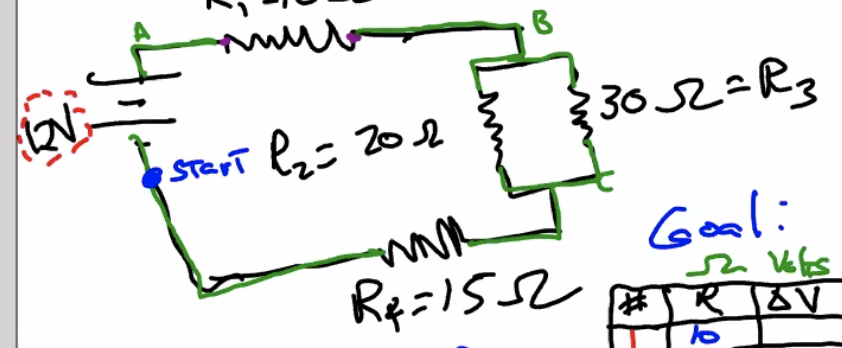
\includegraphics[width=.9\linewidth]{./Screen Shot 2020-09-14 at 10.38.44 AM.png}
\caption{Screen Shot 2020-09-14 at 10.38.44 AM.png}
\end{figure}

So, to calculate the resistance and current at every point o

START at start

\begin{itemize}
\item \(+12\)
\item \(-I_1*10\) (per \(I = \frac{\Delta V}{resistance}\))
\item \(-I_2 * 20\)
\item \(-I_1 * 15\)
\item \(= 0\)
\end{itemize}

\(I_1 - I_2 - I_3 = 0\), per Kirerbab's Second Law.
\end{document}
